%----------------------------------------------------------------------------------------
%	PRESETS AND OPTIONS
%----------------------------------------------------------------------------------------
\documentclass{beamer}
\mode<presentation> {
\usetheme{Madrid} 
\usecolortheme{whale}
\setbeamertemplate{navigation symbols}{}} % remove the navigation symbols

\usepackage{amsmath}
\usepackage{amsthm}
\usepackage{amssymb}
\usepackage{bbold}
\usepackage{ragged2e}
\usepackage{graphicx} % Allows including images
\usepackage{booktabs} % Allows the use of \toprule, \midrule and \bottomrule in tables
\usepackage{pgfplots}
\pgfplotsset{ticks=none}
\tikzset{pointille/.style={dash pattern = on 2pt off 2pt on 6pt off 2pt}}
\tikzset{points/.style={dash pattern = on 1pt off 1pt}}
\tikzset{tirets/.style={dash pattern = on 5pt off 5pt}}

\title[The Ziggurat Method]{The Ziggurat Method} % The short title appears at the bottom of every slide, the full title is only on the title page

\author{Daniel de Souza Severo}
\institute[UofT]
{
University of Toronto\\ % Your institution for the title page
\medskip
\textit{danielsouzasevero@gmail.com} % Your email address
}
\date{\today}



%----------------------------------------------------------------------------------------
%	TITLE AND OVERVIEW
%----------------------------------------------------------------------------------------
\begin{document}

\begin{frame}
\titlepage % Print the title page as the first slide
\end{frame}

\begin{frame}
\frametitle{Overview} % Table of contents slide, comment this block out to remove it
\tableofcontents % Throughout your presentation, if you choose to use \section{} and \subsection{} commands, these will automatically be printed on this slide as an overview of your presentation
\end{frame}

%----------------------------------------------------------------------------------------
%	PRESENTATION SLIDES
%----------------------------------------------------------------------------------------
\section{Introduction}
	\begin{frame} 
		\frametitle{Introduction} 
		This method was originally created by Marsaglia [3]. It has been improved by many including McFarland [2]. This presentation is based on both of these papers.
		\begin{itemize}
			\item Pseudo-random number generators (PRNG’s) are crucial in the context of simulating noise in communication channels.
			\item We present a report on an efficient method for generating pseudo-random samples
from any decreasing probability distribution called the \textbf{Ziggurat Method}.
		\end{itemize}
	\end{frame}

\section{First Glance}
	\begin{frame}
		\frametitle{First Glance} 
		\begin{columns}
			\begin{column}{0.35\linewidth}
				\begin{figure}
					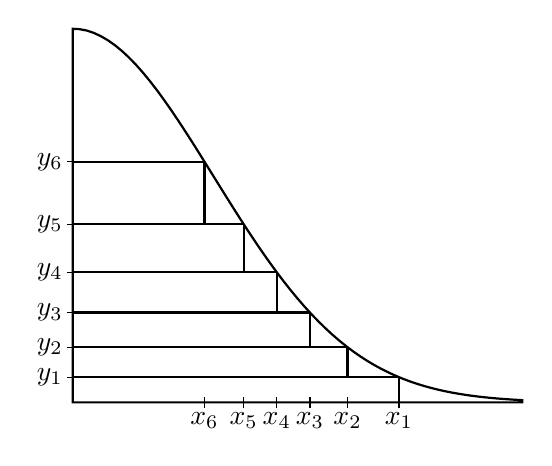
\begin{tikzpicture}
\begin{axis}[samples=65,axis lines=none]    
 	\addplot[thick,domain=0:3.2] {2/sqrt(2*pi)*exp(-x^2/2)}\closedcycle;
 	\addplot [thick,color=black,mark=]coordinates {(2.3221253415052108722, 0.053829996928147945431) (0, 0.053829996928147945431)};
 	\addplot [thick,color=black,mark=]coordinates {(2.3221253415052108722, 0.053829996928147945431) (2.3221253415052108722, 0)};
 	
 	\addplot [thick,color=black,mark=]coordinates {(1.9563286553575721702, 0.11772519145881991813) (0, 0.11772519145881991813)};
 	\addplot [thick,color=black,mark=]coordinates {(1.9563286553575721702, 0.11772519145881991813) (1.9563286553575721702, 0.053829996928147945431)};
 	
	\addplot [thick,color=black,mark=]coordinates {(1.6886556366482920007, 0.19174857271380732284) (0, 0.19174857271380732284)};
 	\addplot [thick,color=black,mark=]coordinates {(1.6886556366482920007, 0.19174857271380732284) (1.6886556366482920007, 0.11772519145881991813)};
 	
	\addplot [thick,color=black,mark=]coordinates {(1.4526281686201162346, 0.27779949937230677675) (0, 0.27779949937230677675)};
 	\addplot [thick,color=black,mark=]coordinates {(1.4526281686201162346, 0.27779949937230677675) (1.4526281686201162346, 0.19174857271380732284)};	
 	
	\addplot [thick,color=black,mark=]coordinates {(1.2169036475136748573, 0.38051921777843910984) (0, 0.38051921777843910984)};
 	\addplot [thick,color=black,mark=]coordinates {(1.2169036475136748573, 0.38051921777843910984) (1.2169036475136748573, 0.27779949937230677675)};	 	
 	
 	\addplot [thick,color=black,mark=]coordinates {(0.93836855027265858619, 0.51372913829813168844) (0, 0.51372913829813168844)};
 	\addplot [thick,color=black,mark=]coordinates {(0.93836855027265858619, 0.51372913829813168844) (0.93836855027265858619, 0.38051921777843910984)};
 	
	\addplot [black, mark = -, nodes near coords=$y_6$,every node near coord/.style={anchor=0}] coordinates {(0, 0.51372913829813168844)};	
 	
 	\addplot [black, mark = -, nodes near coords=$y_5$,every node near coord/.style={anchor=0}] coordinates {(0, 0.38051921777843910984)};
 	
 	\addplot [black, mark = -, nodes near coords=$y_4$,every node near coord/.style={anchor=0}] coordinates {(0, 0.27779949937230677675)}; 	
 	\addplot [black, mark = -, nodes near coords=$y_3$,every node near coord/.style={anchor=0}] coordinates {(0, 0.19174857271380732284)};
 	
 	\addplot [black, mark = -, nodes near coords=$y_2$,every node near coord/.style={anchor=0}] coordinates {(0, 0.11772519145881991813)};
 	
	 \addplot [black, mark = -, nodes near coords=$y_1$,every node near coord/.style={anchor=0}] coordinates {(0, 0.053829996928147945431)}; 	
	 
	 \addplot [black, mark = |, nodes near coords=$x_6$,every node near coord/.style={anchor=90}] coordinates {(0.93836855027265858619, 0)};	
 	
 	\addplot [black, mark = |, nodes near coords=$x_5$,every node near coord/.style={anchor=90}] coordinates {(1.2169036475136748573, 0)};
 	
 	\addplot [black, mark = |, nodes near coords=$x_4$,every node near coord/.style={anchor=90}] coordinates {(1.4526281686201162346, 0)}; 	
 	\addplot [black, mark = |, nodes near coords=$x_3$,every node near coord/.style={anchor=90}] coordinates {(1.6886556366482920007, 0)};
 	
 	\addplot [black, mark = |, nodes near coords=$x_2$,every node near coord/.style={anchor=90}] coordinates {(1.9563286553575721702, 0)};
 	
	 \addplot [black, mark = |, nodes near coords=$x_1$,every node near coord/.style={anchor=90}] coordinates {(2.3221253415052108722, 0)}; 	
 	
\end{axis}
					\end{tikzpicture}
				\end{figure}
			\end{column}
			
			\begin{column}{0.45\linewidth}
				\begin{itemize}
					\item Divide the distribution into simpler regions.
					\item Sample proportional to each region.
				\end{itemize}
			\end{column}
			
		\end{columns}
	\end{frame}
\section{Region Sampling}
\begin{frame}
\frametitle{Region Sampling (1/2)}
	Given a complicated distribution $g$ that encloses an area $A$, how can we create a dataset with distribution $g$ without sampling directly from the density itself?
\begin{figure}[h]
\begin{columns}
\begin{column}{0.45\linewidth}
	\centering
	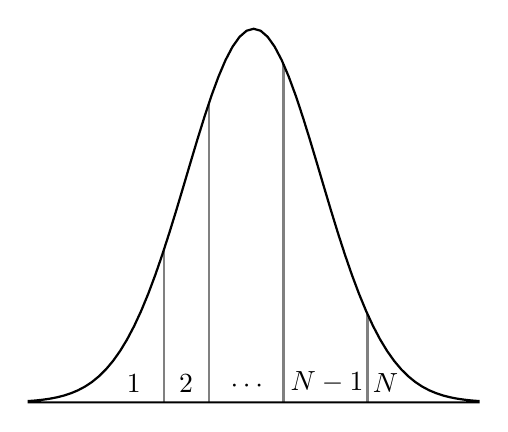
\begin{tikzpicture}
		\begin{axis}[samples=65,axis lines=none]
		\addplot [thick,color=gray,mark=]coordinates {(-0.15, 0.31856) (-0.15, 0)};
		\addplot [thick,color=gray,mark=]coordinates {(-0.3, 0.16219) (-0.3, 0)};
		\addplot [thick,color=gray,mark=]coordinates {(0.1, 0.3609) (0.1, 0)};
		\addplot [thick,color=gray,mark=]coordinates {(0.38, 0.09414) (0.38, 0)};
	 	\addplot[thick,domain=-0.75:0.75,] {1/(2*pi)^0.5*exp(-x^2/0.1)}\closedcycle;
	 	\addplot [black, nodes near coords=$1$] coordinates {(-0.4, 0)};
	 	\addplot [black, nodes near coords=$2$] coordinates {(-0.225, 0)};
	 	\addplot [black, nodes near coords=$\dotsb$,every node near coord/.style={anchor=270}] coordinates {(-0.015, 0)};
		\addplot [black, nodes near coords=$N-1$] coordinates {(0.245, 0)};
	 	\addplot [black, nodes near coords=$N$] coordinates {(0.44, 0)};
 	\end{axis}
\end{tikzpicture}

\label{fig:psampling}
\end{column}

\begin{column}{0.50\linewidth}
\begin{theorem}
	\begin{enumerate}
		\item Divide $A$ into $\{A_i, \dotsb, A_N\}$.
		\item Select $A_i$ with probability $\mu(A_i)$.
		\item Uniformly sample $(x,y)$ from $A_i$.
		\item Return $x$.
	\end{enumerate}
\end{theorem}
\end{column}

\end{columns}
\caption{A general distribution $g$ being divided into $N$ regions $A_i$ with area $\mu(A_i)$.}
\end{figure}
\end{frame}

\begin{frame}
	\frametitle{Region Sampling (2/2)}
	Given a complicated distribution $g$ that encloses an area $A$, how can we create a dataset with distribution $g$ without sampling directly from the density itself?

\begin{theorem}
	\begin{enumerate}
		\item Divide the region $A$ under $g$ into subregions $A_i$ such that $\{A_i, \dotsb, A_N\}$ is a partition\footnote{This means that $A=\bigcup_{i=1}^N A_i$ and $A_i \cap A_j=\emptyset$ for all $i\neq j$.} of $A$.
		\item Randomly select a region $A_i$ with probability proportional to it's area, $\mu(A_i)$.
		\item Uniformly sample a point $p=(x,y)$ from the selected region $A_i$.
		\item Return $x$, since it will have distribution $g$.
	\end{enumerate}
\end{theorem}
\end{frame}
\section{Method}
	\begin{frame}
		\frametitle{Method (1/2)} 
		\begin{columns}
			\begin{column}{0.35\linewidth}
				\begin{figure}
					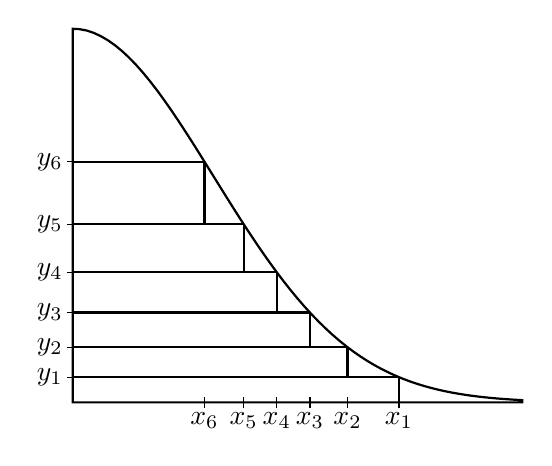
\begin{tikzpicture}
\begin{axis}[samples=65,axis lines=none]    
 	\addplot[thick,domain=0:3.2] {2/sqrt(2*pi)*exp(-x^2/2)}\closedcycle;
 	\addplot [thick,color=black,mark=]coordinates {(2.3221253415052108722, 0.053829996928147945431) (0, 0.053829996928147945431)};
 	\addplot [thick,color=black,mark=]coordinates {(2.3221253415052108722, 0.053829996928147945431) (2.3221253415052108722, 0)};
 	
 	\addplot [thick,color=black,mark=]coordinates {(1.9563286553575721702, 0.11772519145881991813) (0, 0.11772519145881991813)};
 	\addplot [thick,color=black,mark=]coordinates {(1.9563286553575721702, 0.11772519145881991813) (1.9563286553575721702, 0.053829996928147945431)};
 	
	\addplot [thick,color=black,mark=]coordinates {(1.6886556366482920007, 0.19174857271380732284) (0, 0.19174857271380732284)};
 	\addplot [thick,color=black,mark=]coordinates {(1.6886556366482920007, 0.19174857271380732284) (1.6886556366482920007, 0.11772519145881991813)};
 	
	\addplot [thick,color=black,mark=]coordinates {(1.4526281686201162346, 0.27779949937230677675) (0, 0.27779949937230677675)};
 	\addplot [thick,color=black,mark=]coordinates {(1.4526281686201162346, 0.27779949937230677675) (1.4526281686201162346, 0.19174857271380732284)};	
 	
	\addplot [thick,color=black,mark=]coordinates {(1.2169036475136748573, 0.38051921777843910984) (0, 0.38051921777843910984)};
 	\addplot [thick,color=black,mark=]coordinates {(1.2169036475136748573, 0.38051921777843910984) (1.2169036475136748573, 0.27779949937230677675)};	 	
 	
 	\addplot [thick,color=black,mark=]coordinates {(0.93836855027265858619, 0.51372913829813168844) (0, 0.51372913829813168844)};
 	\addplot [thick,color=black,mark=]coordinates {(0.93836855027265858619, 0.51372913829813168844) (0.93836855027265858619, 0.38051921777843910984)};
 	
	\addplot [black, mark = -, nodes near coords=$y_6$,every node near coord/.style={anchor=0}] coordinates {(0, 0.51372913829813168844)};	
 	
 	\addplot [black, mark = -, nodes near coords=$y_5$,every node near coord/.style={anchor=0}] coordinates {(0, 0.38051921777843910984)};
 	
 	\addplot [black, mark = -, nodes near coords=$y_4$,every node near coord/.style={anchor=0}] coordinates {(0, 0.27779949937230677675)}; 	
 	\addplot [black, mark = -, nodes near coords=$y_3$,every node near coord/.style={anchor=0}] coordinates {(0, 0.19174857271380732284)};
 	
 	\addplot [black, mark = -, nodes near coords=$y_2$,every node near coord/.style={anchor=0}] coordinates {(0, 0.11772519145881991813)};
 	
	 \addplot [black, mark = -, nodes near coords=$y_1$,every node near coord/.style={anchor=0}] coordinates {(0, 0.053829996928147945431)}; 	
	 
	 \addplot [black, mark = |, nodes near coords=$x_6$,every node near coord/.style={anchor=90}] coordinates {(0.93836855027265858619, 0)};	
 	
 	\addplot [black, mark = |, nodes near coords=$x_5$,every node near coord/.style={anchor=90}] coordinates {(1.2169036475136748573, 0)};
 	
 	\addplot [black, mark = |, nodes near coords=$x_4$,every node near coord/.style={anchor=90}] coordinates {(1.4526281686201162346, 0)}; 	
 	\addplot [black, mark = |, nodes near coords=$x_3$,every node near coord/.style={anchor=90}] coordinates {(1.6886556366482920007, 0)};
 	
 	\addplot [black, mark = |, nodes near coords=$x_2$,every node near coord/.style={anchor=90}] coordinates {(1.9563286553575721702, 0)};
 	
	 \addplot [black, mark = |, nodes near coords=$x_1$,every node near coord/.style={anchor=90}] coordinates {(2.3221253415052108722, 0)}; 	
 	
\end{axis}
					\end{tikzpicture}
				\end{figure}
			\end{column}
			
			\begin{column}{0.60\linewidth}
				\begin{itemize}
					\item Choose a number $N$ of layers each with area $1/N$.
					\item Define $L_{max}$ as the maximum number of layers that fit under $g$.
					\item Leftover regions represent $1-L_{max}/N$ of the area under $g$.
					\item Apply the Rejection Sampling Algorithm.
				\end{itemize}
			\end{column}
			
		\end{columns}
	\end{frame}
	
		\begin{frame}
		\frametitle{Method (2/2)}
		Example for $N=8$
		\begin{columns}
			\begin{column}{0.35\linewidth}
				\begin{figure}
					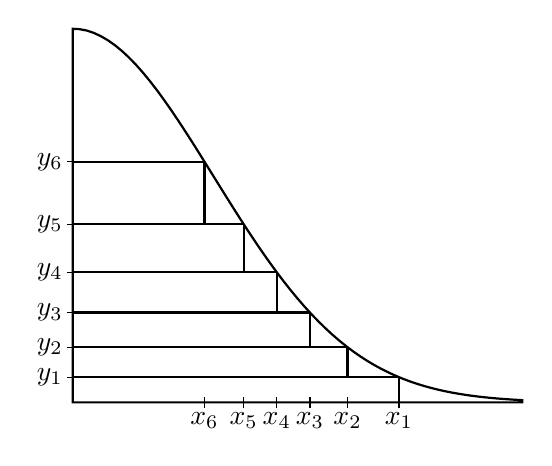
\begin{tikzpicture}
\begin{axis}[samples=65,axis lines=none]    
 	\addplot[thick,domain=0:3.2] {2/sqrt(2*pi)*exp(-x^2/2)}\closedcycle;
 	\addplot [thick,color=black,mark=]coordinates {(2.3221253415052108722, 0.053829996928147945431) (0, 0.053829996928147945431)};
 	\addplot [thick,color=black,mark=]coordinates {(2.3221253415052108722, 0.053829996928147945431) (2.3221253415052108722, 0)};
 	
 	\addplot [thick,color=black,mark=]coordinates {(1.9563286553575721702, 0.11772519145881991813) (0, 0.11772519145881991813)};
 	\addplot [thick,color=black,mark=]coordinates {(1.9563286553575721702, 0.11772519145881991813) (1.9563286553575721702, 0.053829996928147945431)};
 	
	\addplot [thick,color=black,mark=]coordinates {(1.6886556366482920007, 0.19174857271380732284) (0, 0.19174857271380732284)};
 	\addplot [thick,color=black,mark=]coordinates {(1.6886556366482920007, 0.19174857271380732284) (1.6886556366482920007, 0.11772519145881991813)};
 	
	\addplot [thick,color=black,mark=]coordinates {(1.4526281686201162346, 0.27779949937230677675) (0, 0.27779949937230677675)};
 	\addplot [thick,color=black,mark=]coordinates {(1.4526281686201162346, 0.27779949937230677675) (1.4526281686201162346, 0.19174857271380732284)};	
 	
	\addplot [thick,color=black,mark=]coordinates {(1.2169036475136748573, 0.38051921777843910984) (0, 0.38051921777843910984)};
 	\addplot [thick,color=black,mark=]coordinates {(1.2169036475136748573, 0.38051921777843910984) (1.2169036475136748573, 0.27779949937230677675)};	 	
 	
 	\addplot [thick,color=black,mark=]coordinates {(0.93836855027265858619, 0.51372913829813168844) (0, 0.51372913829813168844)};
 	\addplot [thick,color=black,mark=]coordinates {(0.93836855027265858619, 0.51372913829813168844) (0.93836855027265858619, 0.38051921777843910984)};
 	
	\addplot [black, mark = -, nodes near coords=$y_6$,every node near coord/.style={anchor=0}] coordinates {(0, 0.51372913829813168844)};	
 	
 	\addplot [black, mark = -, nodes near coords=$y_5$,every node near coord/.style={anchor=0}] coordinates {(0, 0.38051921777843910984)};
 	
 	\addplot [black, mark = -, nodes near coords=$y_4$,every node near coord/.style={anchor=0}] coordinates {(0, 0.27779949937230677675)}; 	
 	\addplot [black, mark = -, nodes near coords=$y_3$,every node near coord/.style={anchor=0}] coordinates {(0, 0.19174857271380732284)};
 	
 	\addplot [black, mark = -, nodes near coords=$y_2$,every node near coord/.style={anchor=0}] coordinates {(0, 0.11772519145881991813)};
 	
	 \addplot [black, mark = -, nodes near coords=$y_1$,every node near coord/.style={anchor=0}] coordinates {(0, 0.053829996928147945431)}; 	
	 
	 \addplot [black, mark = |, nodes near coords=$x_6$,every node near coord/.style={anchor=90}] coordinates {(0.93836855027265858619, 0)};	
 	
 	\addplot [black, mark = |, nodes near coords=$x_5$,every node near coord/.style={anchor=90}] coordinates {(1.2169036475136748573, 0)};
 	
 	\addplot [black, mark = |, nodes near coords=$x_4$,every node near coord/.style={anchor=90}] coordinates {(1.4526281686201162346, 0)}; 	
 	\addplot [black, mark = |, nodes near coords=$x_3$,every node near coord/.style={anchor=90}] coordinates {(1.6886556366482920007, 0)};
 	
 	\addplot [black, mark = |, nodes near coords=$x_2$,every node near coord/.style={anchor=90}] coordinates {(1.9563286553575721702, 0)};
 	
	 \addplot [black, mark = |, nodes near coords=$x_1$,every node near coord/.style={anchor=90}] coordinates {(2.3221253415052108722, 0)}; 	
 	
\end{axis}
					\end{tikzpicture}
				\end{figure}
			\end{column}
			
			\begin{column}{0.60\linewidth}
\begin{enumerate}
	\item Sample an integer $i$ uniformly between $1$ and $N=8$.
	\item If $i\in[1,L_{max}=6]$, return $x$ uniformly from region $[0,x_i)$. (This represents the layers).
	\item Else, sample an integer $j\in[1,7]$ with probability $p(j)=\mu(A_j)$.
	\begin{enumerate}
		\item If $j=1$, return a sample $x$ from the tail.
		\item Else, apply Rejection Sampling to get a uniform sample $x$ from region $j$.
	\end{enumerate}
\end{enumerate}
			\end{column}
			
		\end{columns}
	\end{frame}
\section{Implementation and Speed Comparison}
\begin{frame}
\frametitle{Implementation and Speed Comparison}
	\begin{itemize}
		\item The Ziggurat algorithm implemented in C for N = 256, is over 4 times
faster than the tradition polar method [1], running on an Intel i7-4790 clocked at 3.60 GHz with 16
GB of RAM.
		\item McFarland [2] has made available all the necessary codes to be used in C, Python and MATLAB. It can be found at \url{https://bitbucket.org/cdmcfarland/fast_prng}.
		\item We have uploaded a Python script that generates all the necessary tables ($x_i$, $y_i=g(x_i)$ and $A_j$) for any given bin size $N$: \url{https://github.com/dsevero/A-Report-on-the-Ziggurat-Method/blob/master/ziggurat/generate_tables.py}
	\end{itemize}
\end{frame}

\section{References}
	
\begin{frame}
\frametitle{References}
\begin{description}
\item[1] George Marsaglia, \textbf{A convenient method for generating normal variables.}, SIAM Rev. 6, 260-264, 1964.
\item[2] Christopher D. McFarland, \textbf{A modified ziggurat algorithm for generating exponentially- and normally-distributed pseudorandom numbers.}, Apr. 2014.
\item[3] George Marsaglia, Wai Wan Tsang, \textbf{A fast, easily implemented method for sampling from decreasing or symmetric unimodal density functions}, SIAM Journ. Scient. and Statis. Computing, 5, 349-359, 1984.
\end{description}
\end{frame}

\section{Appendix}
\begin{frame}


\frametitle{Appendix (1/3)}
Let $I$ be a random variable with distribution $f_I(i)=\mu(A_i)/\mu(A)=\mu(A_i)$. If $P=(X,Y)$ represents the points uniformly sampled in each region, then $f_{P|I}(p|i)=\mathbb{1}\{p \in A_i\}/\mu(A_i)$.\footnote{$\mathbb{1}\{x\}=1$ if $x$ is true and $0$ if it is false.} We can now calculate $f_P(p)=f_{X,Y}(x,y)$:
$$f_P(p)=\sum_i f_I(i)f_{P|I}(p|i)=\sum_i \mu(A_i)\frac{\mathbb{1}\{p \in A_i\}}{\mu(A_i)}=\sum_i \mathbb{1}\{p \in A_i\}$$
A specific point $p$ can only belong to one subregion, since $A_i \cap A_j=\emptyset, \forall i\neq j$. Hence, we have that: 
$$f_P(p)=\sum_i \mathbb{1}\{p \in A_i\} = \mathbb{1}\{p \in A_1\} + \mathbb{1}\{p \in A_2\} + \dotsb + \mathbb{1}\{p \in A_N\} = 1$$
$$f_X(x)=\int_y f_{X,Y}(x,y)dy = \int_0^{g(x)}dy = g(x)$$
\end{frame}

\begin{frame}


\frametitle{Appendix (2/3)}
\begin{figure}[h]
\centering
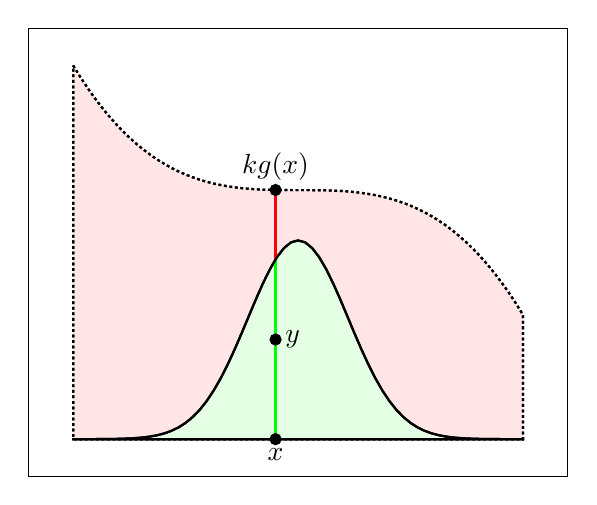
\begin{tikzpicture}
\begin{axis}[samples=65]    
 	\addplot[points,thick,domain=-1:1,fill=red!10] {0.25*(2-x^3)}\closedcycle;
 	\addplot[thick,domain=-1:1,fill=green!10] {1/(2*pi)^0.5*exp(-x^2/0.1)}\closedcycle;
    \addplot [thick,color=red,mark=]coordinates {(-0.1, 0.50025) (-0.1, 0)};
    \addplot [thick,color=green,mark=]coordinates {(-0.1, 0.36) (-0.1, 0)};
    \addplot[thick,domain=-1:1] {1/(2*pi)^0.5*exp(-x^2/0.1)}\closedcycle;
    \addplot[points,thick,domain=-1:1] {0.25*(2-x^3)}\closedcycle; \label{g_label}
	\addplot [black, mark = *, nodes near coords=$kg(x)$,every node near coord/.style={anchor=270}] coordinates {(-0.1, 0.50025)};
	\addplot [black, mark = *, nodes near coords=$y$,every node near coord/.style={anchor=180}] coordinates {(-0.1, 0.2)};
	\addplot [black, mark = *, nodes near coords=$x$,every node near coord/.style={anchor=90}] coordinates {(-0.1, 0)};
    \end{axis}
\end{tikzpicture}
	\caption{RSA rejection/acceptance regions. After sampling $x$ from $g$ (\ref{g_label}) if $y$ falls under curve $h$ (green) then it is stored, otherwise if it is above $h$ (red) it is rejected.}
	\label{fig:RSA}
\end{figure}
\end{frame}


\begin{frame}
\frametitle{Appendix (3/3)}
Define $X \sim f_X(x)\equiv g(x)$ and $Y \sim f_{Y|X}(y|x)=Uniform[0,kg(x)]$.
Now, define $Z=\mathbb{1}\{Y<h(X)\}$ such that if the sample $y$ is under the curve $h$, then $Z$ takes on the value $1$, otherwise $0$.

$$f_{Z|X}(z=1|x)=\frac{h(x)}{kg(x)}$$

Consider now the pair $(X,Z)$ where $(X,Z=1)$ represents the sample points $X$ that we will keep according to the RSA.

$$f_{X,Z}(x,z=1)=f_X(x)f_{Z|X}(z=1|x)=g(x)\frac{h(x)}{kg(x)}=\frac{1}{k}h(x)$$ 

\end{frame}



\end{document}
